


Currently, gender equality barometers, as the Bloomberg Gender Equality Index or the Equileap Ranking, display the result of each company as a single number, score or grade. With this information, a consumer (e.g. an investor) can see which company performs cares about gender equality or which company is "'more"' gender equal than another one. But this one-dimensional approach does not offer a lot more insight.\\
A consumer of such a ranking (e.g. an investor) is probably not only interested that a company makes effort in gender equality, but also \textbf{how} they do.
Moreover, to see how a single number (e.g. the rating result)-which includes a lot of different factors- is composed, it requires quite a bit of investigation.
To address these points, our display solution focuses on a multidimensional approach by means of spider diagrams.\\

\begin{figure}[H]
	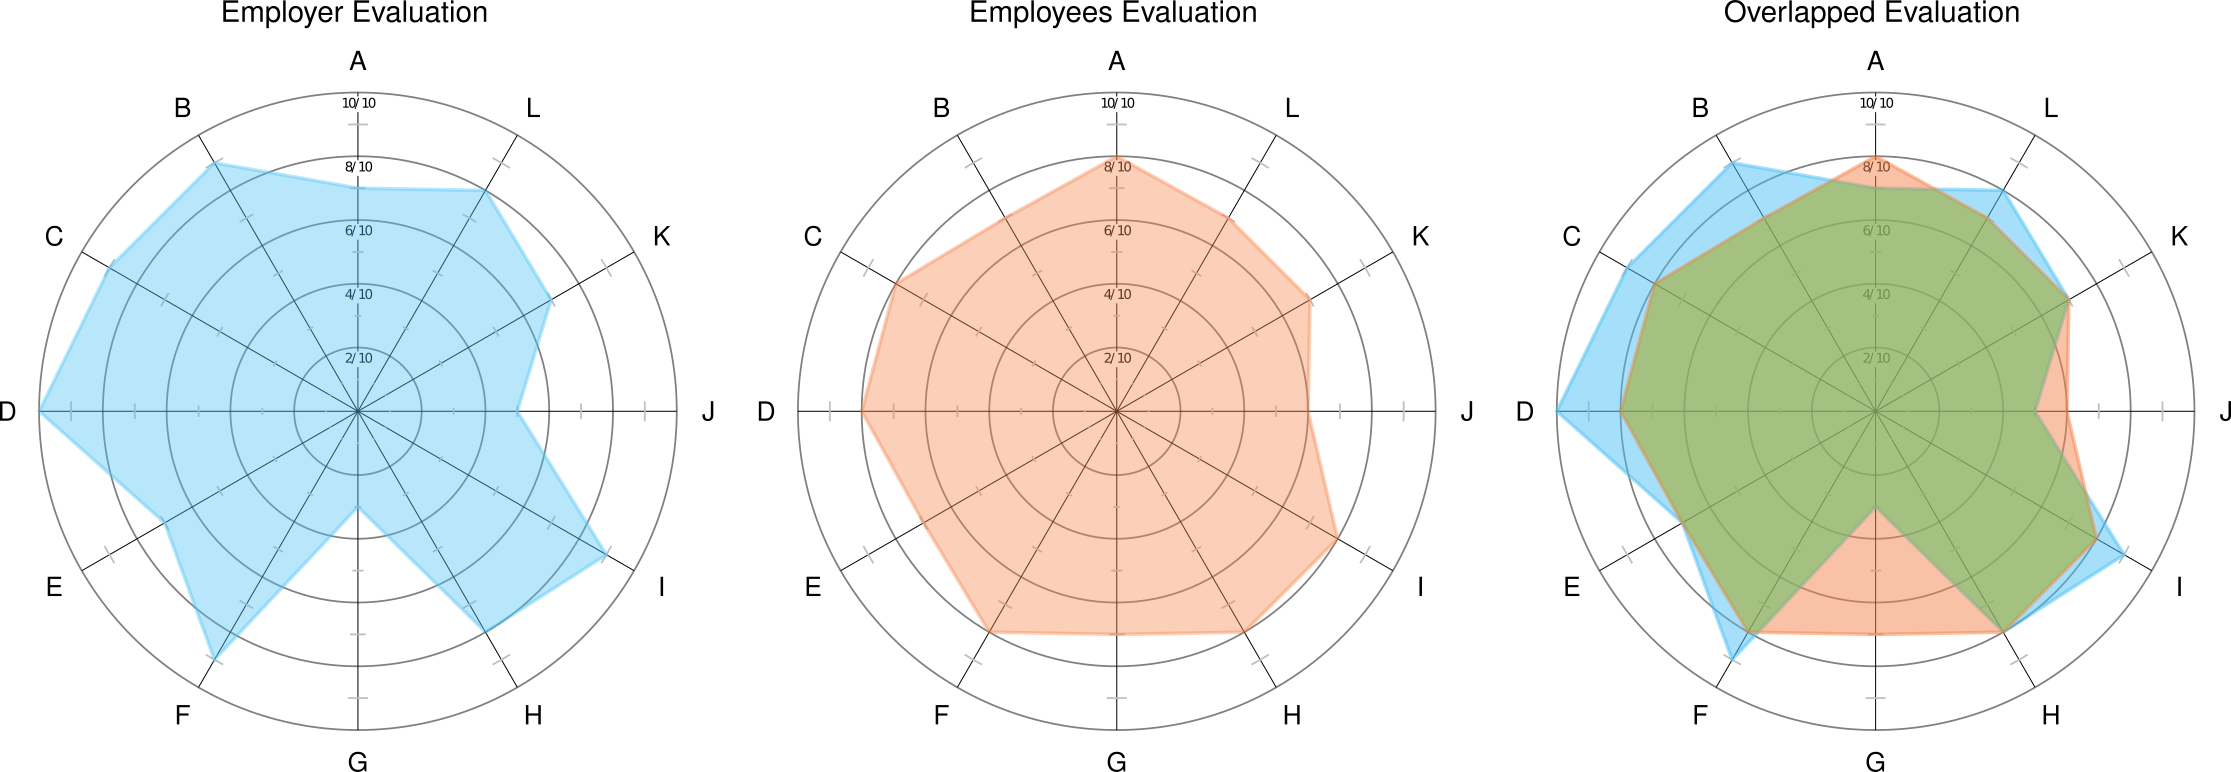
\includegraphics[width=0.95\textwidth]{Bilder/spider-eval}
	\caption{Spider-diagram evaluation example}
	\label{Spider_diagram_evaluation}
\end{figure}

With the spider diagram it is possible to show multiple factors at the same time. One each branch of the diagram a different factor can be displayed (in the figure, the labels 'A - L' represent each one factor.\\
An important in the survey evaluation is to identify the relevant factors which should be included into the spider diagram. These factors could rely on the existing frameworks ( e.g. from Bloomberg or Equileap) or one could come up with new factors based on the surveys. An obvious factor is for sure the difference of salaries between men and women for equal performances.\\
 
Due to the settings of the surveys, there will be data from the employer survey which can not be caputered by the employee survey and vice versa. For example, the employer can deliver factual data, whereas the employee can express his personal impressions and experiences of the daily work life. This data can be boundled in the \textit{non-intersecting-data category}. Nevertheless, concerns, which are addressed in both surveys can be compared. This data can be boundled in the \textit{intersecting-data category}.\\
As shown schematically in the figure above, these two categories can be in an straigtforward manner with spider diagrams. On the one hand, the \textit{non-intersecting-data category}, there could be a spider diagram for the employer survey as well as the employee survey. On the other hand, a spider diagram with the \textit{intersecting-data category} could present the factors, where data from both sides is displayed.\\

The overlapping in the spider diagram of the \textit{intersecting-data category} can serve as an indicator of data-validity. When a company provides wrong data, then this would result in a smaller overlapp. One has to take into account, that people could be forced by the company to give certain answers to gain a competitve advantage. As this problem is too extensive, we consider it as a further point to investigate on.\\

Since spider diagrams are widely known, and the display solution is easy to read. Due to the fact that the diagram displays more than a number as the other ratings, it is a nice tool to gain additional, comprehensible insight into the efforts a company does in the field of gender equality.\\

Because the data from the evaluations is open accessible on IPFS, the diagrams can easily be generated and fetched from these places and be displayed via a website or an app.\\


